% !TEX root = ../metrics_hse_exams.tex

\subsection{Контрольная работа 1}

\begin{enumerate}
\item (20 баллов) Была оценена регрессия вида

\[
Y_i = \beta_1 + \beta_2X_{i1} + \beta_3X_{i2} + \beta_4X_{i3} + \beta_5X_{i4} + \varepsilon_i.
\]

Результаты оценивания регрессии представлены в таблице ниже.

\begin{figure}[h]
	\begin{center}
				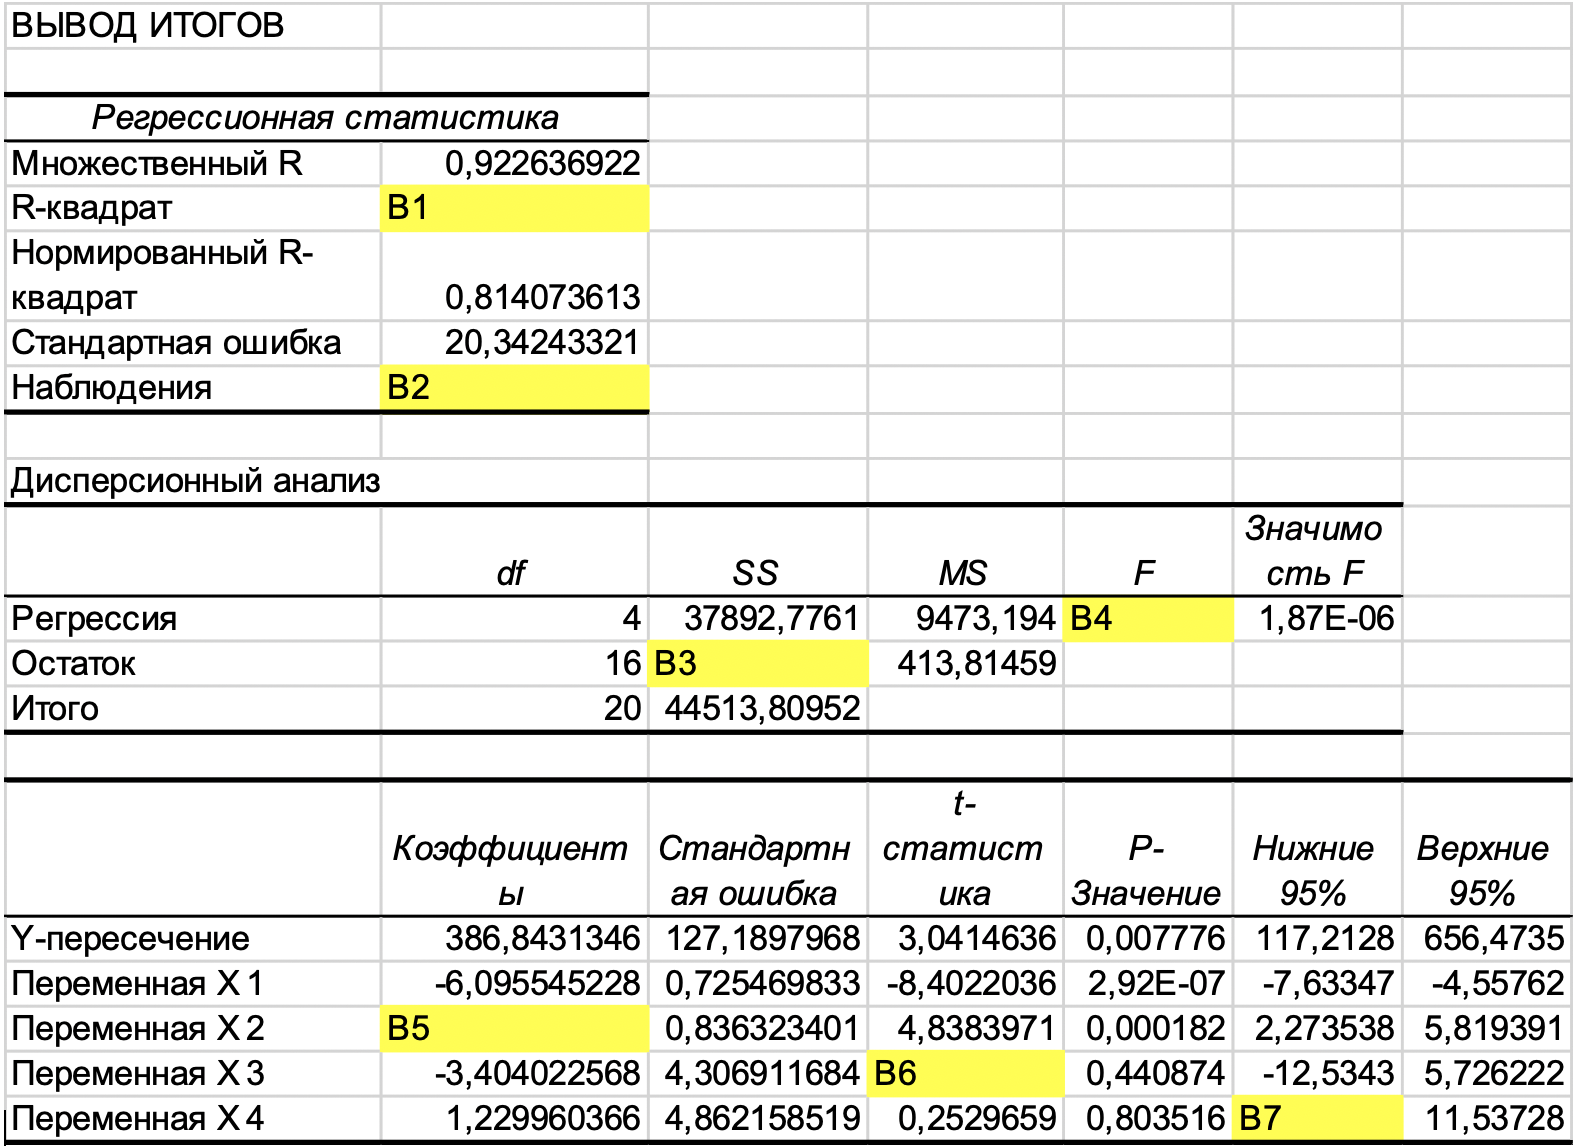
\includegraphics[scale=0.5]{figures/2022-2023_kr1.png}
	\end{center}
\end{figure}

\begin{enumerate}
\item (2 балла) Найдите значение B5.
\item (2 балла) Выпишите оцененное уравнение регрессии.
\item (2 балла) Найдите значение B1.
\item (2 балла) Найдите значение B2.
\item (2 балла) Найдите значение B3.
\item (2 балла) Найдите значение B4.
\item (2 балла) Найдите значение B6.
\item (2 балла) Найдите значение B7.
\item (4 балла) Сделайте вывод о значимости коэффициентов регрессии на уровне значимости 5\% и проинтерпретируйте полученные результаты.
\end{enumerate}

\item (20 баллов) Исследуется зависимость реального дохода на душу населения $y$ (в тыс.долл.) от процента рабочей силы, занятой в сельском хозяйстве, $x_1$ и среднего уровня образования населения в возрасте после 25 лет $x_2$ (число лет, проведенных в учебных заведениях) для 5 развитых стран в 2001 году. По имеющимся данным была оценена следующая модель регрессии:

\[
y_i = \beta_1 + \beta_2x_{i1} + \beta_3x_{i2} + \varepsilon_i.
\]

При этом известно, что

\[
X' X =  \begin{pmatrix}
5 & 3 & 1 \\
3 & 3 & 1 \\
1 & 1 & 1 \\
\end{pmatrix}, \quad (X' X)^{-1} =  \begin{pmatrix}
0.5 & -0.5 & 0 \\
-0.5 & 1 & -0.5 \\
0 & -0.5 & 1.5 \\
\end{pmatrix}, 
\]
\[
X'y =\begin{pmatrix}
15 \\
11 \\
4 
\end{pmatrix}, e'e = 6.5.
\]

\begin{enumerate}
\item (3 балла) Найдите МНК-оценки для параметров модели регрессии.
\item (3 балла) Проинтерпретируйте результаты регрессии.
\item (3 балла) Определите $\widehat{\sigma}^2_{\varepsilon}$, $\widehat{\sigma}^2_{\hb_2}$ и $\widehat{\sigma}^2_{\hb_3}$.
\item (3 балла) Постройте 95\%-ый доверительный интервал для $\beta_2$.
\item (3 балла) Проверьте на 5\%-ом уровне значимости гипотезу о том, что $\beta_2 = 0$ и $\beta_3 = 0$.
\item (2 балла) Спрогнозируйте реальный доход на душу населения для страны, в которой процент рабочей силы, занятой в сельском хозяйстве, составляет 7\% и средний уровень образования населения в возрасте после 25 лет составляет 12 лет.
\item (3 балла) Постройте 95\%-ый доверителный интервал для прогноза из предыдущего пункта.
\end{enumerate}

\item (10 баллов) Рассмотрим следующую регрессионную модель зависимости логарифма заработной платы $\ln (W)$ от уровня образования $Edu$ и опыта работы $Exp$, $Exp^2$:
 
\[
\widehat{\ln (W)_i} = \hb_0 + \hb_1 Edu_i + \hb_2 Exp_i + \hb_3 Exp^2_i.
\]

Модель регрессии была отдельно оценена по выборкам из 20 мужчин и 20 женщин, и
были получены остаточные суммы квадратов $RSS_{male} = 49.4$ и $RSS_{female} = 44.1$ Остаточная сумма квадратов в регрессии, оцененной по объединенной выборке ($RSS_{pooled}$), равна 105.5. Протестируйте на 5\%-ом уровне значимости гипотезу об отсутствии дискриминации в оплате труда между мужчинами и женщинами.

\item (10 баллов) Рассмотрим оценку вида $\tilde\beta = (X'X+rD)^{-1}X'y$ для вектора коэффициентов регрессионного уравнения $y = X\beta + \varepsilon$, где $D$ – диагональная $k \times k$ матрица, состоящая из диагональных элементов матрицы $X'X$.

\begin{enumerate}
\item (5 баллов) Найдите математическое ожидание оценки $\tilde\beta$.
\item (5 баллов) Найдите матрицу ковариаций оценки $\tilde\beta$.
\end{enumerate}
\end{enumerate}
